% Este trabalho está licenciado sob a Licença Atribuição-CompartilhaIgual 4.0 Internacional Creative Commons. Para visualizar uma cópia desta licença, visite http://creativecommons.org/licenses/by-sa/4.0/deed.pt_BR ou mande uma carta para Creative Commons, PO Box 1866, Mountain View, CA 94042, USA.

\chapter{Linguagem de Programação}\label{cap_lingua}
\thispagestyle{fancy}

\section{Computador}\label{cap_lim_sec_computador}

\begin{flushright}
  [YouTube] | [Vídeo] | [Áudio] | [Contatar]
\end{flushright}

Um computador\footnote{Consulte \href{https://pt.wikipedia.org/wiki/Computador}{Wikipédia: Computador} para uma introdução sobre a história e outras questões sobre computadores.} é um \emph{sistema computacional} de elementos físicos (\emph{hardware}) e elementos lógicos (\emph{software}).

O \emph{hardware} são suas partes mecânicas, elétricas e eletrônicas como: fonte de energia, teclado, mouse/painel tátil, monitor/tela, dispositivos de armazenagem de dados (HDD, {\it hard disk drive}; SSD, {\it solid-state drive}; RAM, {\it random-access memory}; etc.), dispositivos de processamento (CPU, {\it central processing unit}, GPU, {\it graphics processing unit}), conectores de dispositivos externos (microfone, caixa de som, fone de ouvido, USB, etc.), placa mãe, etc..

O \emph{software} é toda a informação processada pelo computador, qualquer código executado e qualquer dado usado nas computações.

\begin{figure}[H]
  \centering
  \includegraphics[width=\textwidth]{./cap_lingua/dados/fig_arqVonNeumann/main}
  \caption[Arquitetura de von Neumann]{Arquitetura de computador de von Neumann.}
  \label{cap_lim_sec_computador:fig:arqVonNeumann}
\end{figure}

Os computadores que comumente utilizamos seguem a arquitetura de John von Neumann\footnote{John von Neumann, 1903 - 1957, matemático húngaro, naturalizado estadunidense. Fonte: \href{https://pt.wikipedia.org/wiki/John_von_Neumann}{Wikipédia}.}, que consiste em dispositivo(s) de entrada de dados, unidade(s) de processamento, unidade(s) de memória e dispositivo(s) de saída de dados (Figura~\ref{cap_lim_sec_computador:fig:arqVonNeumann}).

\begin{itemize}
\item \emph{Dispositivos de entrada e saída}

  São elementos do computador que permitem a comunicação humana (usuária(o)) com a máquina.

  \begin{itemize}
  \item \emph{Dispositivos de entrada}

    São elementos que permitem o fluxo de informação da(o) usuária(o) para a máquina. Exemplos são: teclado, mouse/painel tátil, microfone, etc.

  \item \emph{Dispositivos de saída}

    São elementos que permitem o fluxo de informação da máquina para a(o) usuária(o). Exemplos são: monitor/tela, alto-falantes, luzes espia, etc.
  \end{itemize}

\item \emph{Unidade central de processamento}

  A \emph{CPU} (do inglês, {\it Central Processing Unit}) é o elemento de processa as informações e é composta de \emph{unidade de controle}, \emph{unidade lógica e aritmética} e de \emph{memória cache}.

  \begin{itemize}
  \item \emph{Unidade de controle}

    Coordena as execuções do processador: busca e decodifica instruções, lê e escreve no {\it cache} e controla o fluxo de dados.

  \item \emph{Unidade lógica/aritmética}

    Executa as instruções operações lógicas e aritméticas, por exemplo: executar a adição, multiplicação, testar se dois objetos são iguais, etc.

  \item \emph{Memória cache}

    Memória interna da CPU muito mais rápida que as memórias RAM e dispositivos e armazenamento HDD/SSD. É um dispositivo de memória de pequena capacidade e é utilizada como memória de curto prazo e diretamente acessada.
  \end{itemize}

\item \emph{Unidades de memória}

  As unidades de memória são elementos que permitem o armazenamento de dados/objetos. Como memória principal tem-se a \emph{ROM} (do inglês, {\it Read Only Memory}) e a \emph{RAM} (do inglês, {\it Random Access Memory}) e como memória de massa/secundária tem-se HDD, SSD, entre outras.

\item \emph{Memória ROM}

  A memória ROM é utilizada para armazenamento de dados/objetos necessários para dar início ao funcionamento do computador. Por exemplo, é onde a BIOS (dos inglês, {\it Basic Input/Output System}, Sistema Básico de Entrada e Saída) é armazenada. Ao ligarmos o computador este programa é iniciado e é responsável por fazer o gerenciamento inicial dos diversos dispositivos do computador e carregar o \emph{sistema operacional} (conjunto de programas cuja função é de gerenciar os recursos do computador e controlar a execução de programas).

\item \emph{Memória RAM}

  Memória de acesso rápido utilizada para dados/objetos de uso frequente durante a execução de programas. É uma memória volátil, i.e. toda a informação guardada nela é perdida quando o computador é desligado.

\item \emph{Memória de massa/secundária}

  Memória de massa ou secundária são usadas para armazenar dados/objetos por período longo. Normalmente, são dispositivos HDD ou SSD, os dados/objetos são guardados mesmo que o computador seja desligado e contém grande capacidade de armazenagem.   
\end{itemize}

Os \emph{software} são os elementos lógicos de um sistema computacional, são programas de computadores que contém as instruções que gerenciam o \emph{hardware} para a execução de tarefas específicas, por exemplo, imprimir um texto, gravar áudio/vídeo, resolver um problema matemático, etc. Programar é o ato de criar programas de computadores.

\subsection{Linguagem de programação}

As informações fluem no computador codificadas como registros de {\it bits}\footnote{Usualmente de tamanho $64$-{\it bits}.} (sequência de zeros ou uns). Há registros de instrução e de dados. Programar diretamente por registros é uma tarefa muito difícil, o que levou ao surgimento de linguagens de programação. Uma \emph{linguagem de programação}\footnote{Código de programação, código de máquina ou linguagem de máquina.} é um método padronizado para escrever instruções para execução de tarefas no computador. As instruções escritas em uma linguagem são interpretadas e/ou compiladas por um software (interpretador ou compilador) da linguagem que decodifica as instruções em registros de instruções e dados, os quais são efetivamente executados na máquina.

Existem várias linguagens de programação disponíveis e elas são classificadas por diferentes características. Uma \emph{linguagem de baixo nível} (por exemplo, \href{https://pt.wikipedia.org/wiki/Linguagem_assembly}{Assembly}) é aquela que se restringe às instruções executadas diretamente pelo processador, enquanto que uma \emph{linguagem de alto nível} contém instruções mais complexas e abstratas. Estas contém sintaxe mais próxima da linguagem humana natural e permitem a manipulação de objetos mais abstratos. Exemplos de linguagens de alto nível são: \href{https://pt.wikipedia.org/wiki/BASIC}{Basic}, \href{https://pt.wikipedia.org/wiki/Java\_(linguagem\_de\_programa\%C3\%A7\%C3\%A3o)}{Java}, \href{https://pt.wikipedia.org/wiki/JavaScript}{Javascript}, \href{https://pt.wikipedia.org/wiki/MATLAB}{MATLAB}, \href{https://pt.wikipedia.org/wiki/PHP}{PHP}, \href{https://pt.wikipedia.org/wiki/R\_(linguagem_de_programa\%C3\%A7\%C3\%A3o)}{R}, \href{https://pt.wikipedia.org/wiki/C\%2B\%2B}{C/C++}, {\python}, etc.

Em geral, não existe uma melhor linguagem, cada uma tem suas características que podem ser mais ou menos adequadas conforme o programa que se deseja desenvolver. Por exemplo, para um site de internet, linguagens como \href{https://pt.wikipedia.org/wiki/JavaScript}{Javascript} e \href{https://pt.wikipedia.org/wiki/PHP}{PHP} são bastante úteis, mas não no desenvolvimento de modelagem matemática e computacional. Nestes casos, \href{https://pt.wikipedia.org/wiki/C\%2B\%2B}{C/C++} é uma linguagem mais apropriada por conter várias estruturas de programação que facilitam a modelagem computacional de problemas científicos. Agora, \href{https://pt.wikipedia.org/wiki/R\_(linguagem_de_programa\%C3\%A7\%C3\%A3o)}{R} é uma linguagem de alto nível com diversos recursos dedicados às áreas de ciências de dados e estatística. Usualmente, utiliza-se mais de uma linguagem no desenvolvimento de programas mais avançados. A ideia é de explorar o melhor de cada linguagem na criação de programas eficientes na resolução dos problemas de interesse.

Nestas notas de aula, {\python} é a linguagem escolhida para estudarmos algoritmos e programação. Trata-se de uma linguagem de alto nível, \emph{interpretada}, \emph{dinâmica} e \emph{mutiparadigma}. Foi lançada por Guido van Rossum\footnote{Guido van Rossum, 1956-, matemático e programador de computadores holandês. Fonte: \href{https://pt.wikipedia.org/wiki/Guido\_van\_Rossum}{Wikipédia}.} em 1991 e, atualmente, é desenvolvida de forma comunitária, aberta e gerenciada pela ONG \href{https://pt.wikipedia.org/wiki/Python_Software_Foundation}{Python Software Foundation}. A linguagem foi projetada para priorizar a legibilidade do código. Parte da filosofia da linguagem é descrita pelo poema \href{https://pt.wikipedia.org/wiki/Zen_de_Python}{The Zen of Python}. Pode-se lê-lo pelo {\it easter egg} {\python}:
\begin{lstlisting}
  >>> import this
\end{lstlisting}

\begin{itemize}
\item Linguagem interpretada

  {\python} é uma linguagem interpretada. Isso significa que o \emph{código-fonte} escrito em linguagem {\python} é interpretado por um programa (interpretador {\python}). Ao executar-se um código, o interpretador lê uma linha do código, decodifica-a como registros para o processador que os executa. Executada uma linha, o interpretador segue para a próxima até o código ter sido completadamente executado.

\item Linguagem compilada

  Em uma linguagem compilada, como \href{https://pt.wikipedia.org/wiki/C\%2B\%2B}{C/C++}, há um programa chamado de \emph{compilador} (em inglês, {\it compiler}) e outro de \emph{ligador} (em inglês, {\it linker}). O primeiro, cria um programa-objeto a partir do código e o segundo gerencia sua ligação com eventuais bibliotecas computacionais que ele possa depender. O programa-objeto (também chamado de executável) pode então ser executado pela máquina.
\end{itemize}

Em geral, a execução de um programa compilado é mais rápida que a de um código interpretado. De forma simples, isso se deve ao fato de que nesse a interpretação é feita toda de uma vez e não precisa ser refeita na execução de cada linha de código, como no segundo caso. Por outro lado, a compilação de códigos-fonte grandes pode ser bastante demorada fazendo mais sentido quando ele é compilado uma vez e o programa-objeto executado várias vezes. Além disso, linguagens interpretadas podem usar bibliotecas de programas pré-compiladas. Com isso, pode-se alcançar um bom balanceamento entre tempo de desenvolvimento e de execução do código.

O interpretador {\python} também pode ser usado para compilar o código para um arquivo \emph{bytecode}, este é executado muito mais rápido do que o código-fonte em si, pois as interpretações necessárias já foram feitas. Mais adiante, vamos estudar isso de forma mais detalhada.

\begin{itemize}
\item Linguagem de tipagem dinâmica

  {\python} é uma linguagem de tipagem dinâmica. Nela, os dados não precisam ser explicitamente tipificados no código-fonte e o interpretador os tipifica com base em regras da própria linguagem. Ao executar operações com os dados, o interpretador pode alterar seus tipos de forma dinâmica.

\item Linguagem de tipagem estática

  \href{https://pt.wikipedia.org/wiki/C\%2B\%2B}{C/C++} é um exemplo de uma linguagem de tipagem estática. Em tais linguagens, os dados devem ser explicitamente tipificados no código-fonte com base nos tipos disponíveis. A retipificação pode ocorrer, mas precisa estar explicitamente definida no código.
\end{itemize}

Existem vários \emph{paradigmas de programação} e a linguagem {\python} é multiparadigma, i.e. permite a utilização de mais de um no código-fonte. Exemplos de paradigmas de programação são: \emph{estruturada}, \emph{orientada a objetos}, \emph{orientada a eventos}, etc.. Na maior parte destas notas de aulas, vamos estudar algoritmos para linguagens de programação estruturada. Mais ao final, vamos introduzir aspectos de linguagens orientada a objetos. Estes são paradigmas de programação fundamentais e suas estruturas são importantes na programação com demais paradigmas disponíveis em programação de computadores.

\subsection{Instalação e execução}

{\python} é um \emph{software aberto}\footnote{Consulte a licença de uso em \url{https://docs.python.org/3/license.html}.} e está disponível para vários sistemas operacionais ({\linux}, macOS, Windows, etc.) no seu site oficial
\begin{center}
  \url{https://www.python.org/}
\end{center}
Também, está disponível (gratuitamente) na loja de aplicativos dos sistemas operacionais mais usados. Esta costuma ser a forma mais fácil de instalá-lo na sua máquina, consulte a loja de seus sistema operacional. Ainda, há plataformas e IDEs\footnote{IDE, do inglês, {\it Integrated Development enviroment}, ambiente de desenvolvimento integrado} {\python} disponíveis, consulte, como por exemplo, \href{https://www.anaconda.com/}{Anaconda}.

A execução de um código {\python} pode ser feita de várias formas.

\begin{itemize}
\item \emph{Execução iterativa via terminal}

  Em terminal {\python} pode-se executar instruções/comandos de forma iterativa. Por exemplo:
  \begin{lstlisting}
    >>> print('Olá, mundo!')
    Olá, mundo!
    >>> 
  \end{lstlisting}

  O símbolo \lstinline+>>>+ denota o \emph{prompt de entrada}, onde uma instrução {\python} pode ser digitada. Após digitar, o comando é executada teclando \lstinline+<ENTER>+. Caso o comando tenha alguma saída de informação, como no caso acima, esta aparecerá, por padrão, no \emph{prompt de saída}, logo abaixo a linha de comando executada. Um novo símbolo de prompt de entrada aparece ao términa da execução anterior.

\item \emph{Execução de um {\it script}}

  Para códigos com várias linhas de instruções é mais adequado utilizar um aquivo de {\it script} {\python}. Usando-se um editor de texto ou um IDE ditam-se as linhas de comando em um arquivo \lstinline+.py+. Então, {\it script} pode ser executado em um terminal de seu sistema operacional utilizando-se o interpretador {\python}. Por exemplo, assumindo que o código for salvo do arquivo \lstinline+path_to_arq/arq.py+, pode-se executá-lo em um terminal do sistema com
  \begin{lstlisting}
    $ python3 path_to_arq/arq.py 
  \end{lstlisting}%$
  

  IDEs para {\python} fornecem uma ambiente integrado, contendo um campo para escrita do código e terminal {\python} integrado. Consulte, por exemplo, o IDE {\spyder}:
  \begin{center}
    \url{https://www.spyder-ide.org/}
  \end{center}

\item \emph{Execução em um {\it notebook}}

  {\it Notebooks} {\python} são uma boa alternativa para a execução de códigos em um ambiente colaborativo/educativo. Por exemplo, {\jupyter} é um notebook que roda em navegadores de internet. Sua estrutura e soluções também são encontradas em notebooks online (de uso gratuito limitado) como {\colab} e {\kaggle}.  
\end{itemize}

\subsection{Exercícios}

\begin{exer}
  Verifique qual a versão do sistema operacional que está utilizado em seu computador.
\end{exer}
\begin{resp}
  Dica: Em {\linux}, \lstinline+$ uname --all+ ou \lstinline+$ cat /etc/version+.
\end{resp}

\begin{exer}
  Verifique os seguintes elementos de seu computador:
  \begin{enumerate}[a)]
  \item CPUs
  \item Placa(s) gráfica(s)
  \item Memória RAM
  \item Armazenamento HDD/SSD.
  \end{enumerate}
\end{exer}
\begin{resp}
  Dica: Em {\linux}: \lstinline*$ lshw*%$
\end{resp}

\begin{exer}
  Verifique como entrar na \lstinline+BIOS+ de seu computador. Atenção! Não faça  e salve nenhuma alteração, caso não saiba o que está fazendo. Modificações na \lstinline+BIOS+ podem impedir que seu computador funcione normalmente, inclusive, impedir que você inicialize seu sistema operacional.
\end{exer}
\begin{resp}
  Dica: cada computador tem sua forma de acessar a \lstinline+BIOS+. Verifique o manual ou busque na internet pela marca e modelo de seu computador.
\end{resp}

\begin{exer}
  Instale {\python} no seu computador (caso ainda não tenha feito) e abra um terminal {\python}. Nele, escreva uma linha de comando que imprima no prompt de saída a frase ``Olá, meu Python!''.
\end{exer}
\begin{resp}
\begin{lstlisting}
>>> print('Olá, meu Python!')
Olá, meu Python!
>>> 
\end{lstlisting}
\end{resp}

\begin{exer}
  Instale o {\spyder} no seu computador (caso ainda não tenha feito) e use-o para escrever o seguinte {\it script}
\begin{lstlisting}
import math as m
print(f'Número pi = {m.pi}')
print(f'Número de Euler e = {m.e}')
\end{lstlisting}
  Também, execute o {\it script} diretamente em um terminal de seu sistema operacional.
\end{exer}

\begin{exer}
  Use um {\it notebook} {\python} para escrever e executar o código do exercício anterior.
\end{exer}
\begin{resp}
  Dica: use um notebook online {\colab}, {\kaggle} ou {\jupyter}.
\end{resp}

\section{Algoritmos e Programação}\label{cap_lingua_sec_algoprog}

\emph{Programar} é criar um programa (um {\it software}) para ser executado em computador. Para isso, escreve-se um código em uma linguagem computacional (por exemplo, em {\python}), o qual é interpretado/compilado para gerar o programa final. Linguagens computacionais são técnicas, utilizam uma sintaxe simples, precisa e sem ambiguidades. Ou seja, para criarmos um programa com um determinado objetivo, precisamos escrever um código computacional técnico, que siga a sintaxe da linguagem escolhida e sem ambiguidades.

Um \emph{algoritmo} pode ser definido uma sequencia ordenada e sem ambiguidade de passos para a resolução de um problema. Por exemplo, o cálculo da área de um triângulo de base e altura definida por ser feita com o seguinte algoritmo:
\begin{enumerate}
\item Informe o valor da base $b$.
\item Informe o valor da base $h$.
\item $\displaystyle a \leftarrow \frac{b\cdot h}{2}$.
\item Imprima o valor de $a$.
\end{enumerate}

\emph{Algoritmos para a programação são pensados para serem facilmente transformados em códigos computacionais}. Por exemplo, o algoritmo acima pode ser escrito em {\python} como segue:
\begin{lstlisting}
b = float(input('Informe o valor da base.\n'))
h = float(input('Informe o valor da altura.\n'))
# cálculo da área
a = b*h/2
print(f'Área = {a}')
\end{lstlisting}

Para criar um programa para resolver um dado problema, começamos desenvolvendo um algoritmo para resolvê-lo, este algoritmo é implementado na linguagem computacional escolhida, a qual gera o programa final. Aqui, o passo mais difícil costuma ser o desenvolvimento do algoritmo. Precisamos pensar em como podemos resolver o problema de interesse em uma sequência de passos ordenada e sem ambiguidades para que possamos implementá-los em computador.

Um algoritmo deve ter as seguintes propriedades:
\begin{itemize}
\item Cada passo deve estar bem definido, i.e. não pode conter ambiguidades.
\item Cada passo deve contribuir de forma efetiva na solução do problema.
\item Deve ter número finito de passos que podem ser computados em um tempo finito.
\end{itemize}

\begin{obs}
  A primeira pessoa a publicar um algoritmo para programação foi Augusta Ada King\footnote{Augusta Ada King, 1815 - 1852, matemática e escritora inglesa. Fonte: \href{https://pt.wikipedia.org/wiki/Ada_Lovelace}{Wikipédia}.}. O algoritmo foi criado para computar os \href{https://pt.wikipedia.org/wiki/N\%C3\%BAmeros\_de\_Bernoulli}{números de Bernoulli}\footnote{Jacob Bernoulli, 1655-1705, matemático suíço. Fonte: \href{https://pt.wikipedia.org/wiki/Jakob_Bernoulli}{Wikipédia}.}.
\end{obs}


\subsection{Fluxograma}

Fluxograma é uma representação gráfica de um algoritmo. Entre outras, usam-se as seguintes formas para representar tipos de ações a serem executadas:
\begin{itemize}
\item {\bf Terminal}: início ou final do algoritmo.
  \begin{center}
    \includegraphics{./cap_lingua/dados/fig_fluxograma/terminal}
  \end{center}  
\item {\bf Linha de fluxo}: direciona para a próxima execução.
  \begin{center}
    \includegraphics{./cap_lingua/dados/fig_fluxograma/linha}
  \end{center}
\item {\bf Entrada}: leitura de informação/dados.
  \begin{center}
    \includegraphics{./cap_lingua/dados/fig_fluxograma/entrada}
  \end{center}  
\item {\bf Processo}: ação a ser executada.
  \begin{center}
    \includegraphics{./cap_lingua/dados/fig_fluxograma/processo}
  \end{center}
\item {\bf Decisão}: ramificação do processamento baseada em uma condição.
  \begin{center}
    \includegraphics{./cap_lingua/dados/fig_fluxograma/decisao}
  \end{center}
\item {\bf Saída}: impressão de informação/dados.
\end{itemize}

\begin{ex}
  O \href{https://en.wikipedia.org/wiki/Methods_of_computing_square_roots#Heron's_method}{método de Heron}\footnote{Heron de Alexandria, 10 - 80, matemático e inventor grego. Fonte: \href{https://pt.wikipedia.org/wiki/Heron\_de\_Alexandria}{Wikipédia}.} é um algoritmo para o cálculo aproximado da raiz quadrada de um dado número $x$, i.e. $\sqrt{x}$. Consiste na iteração
  \begin{align}
    s^{(0)} &= \text{approx. inicial},\\
    s^{(i+1)} &= \frac{1}{2}\left(s^{(i)} + \frac{x}{s^{(i)}}\right),
  \end{align}
  para $i=0,1,2,\ldots,n$, onde $n$ é o número de iterações calculadas.

  Na sequência, temos um algoritmo e seus fluxograma e código {\python} para computar a quarta aproximação de $\sqrt{x}$, assumindo $s^{(0)} = x/2$ como aproximação inicial.

  \begin{itemize}
  \item {\bf Algoritmo}
    \begin{enumerate}
    \item Entre o valor de $x$.
    \item Se $x\geq 0$, faça:
      \begin{enumerate}
      \item $s \leftarrow x/2$
      \item Para $i = 0,1,2,3$, faça:
        \begin{enumerate}
        \item $s \leftarrow (s + x/s)/2$.
        \end{enumerate}
      \item Imprime o valor de $s$.
      \end{enumerate}
    \item Senão, faça:
      \begin{enumerate}
      \item Imprime mensagem ``Não existe!''.
      \end{enumerate}
    \end{enumerate}

  \item {\bf Fluxograma}

    \begin{center}
      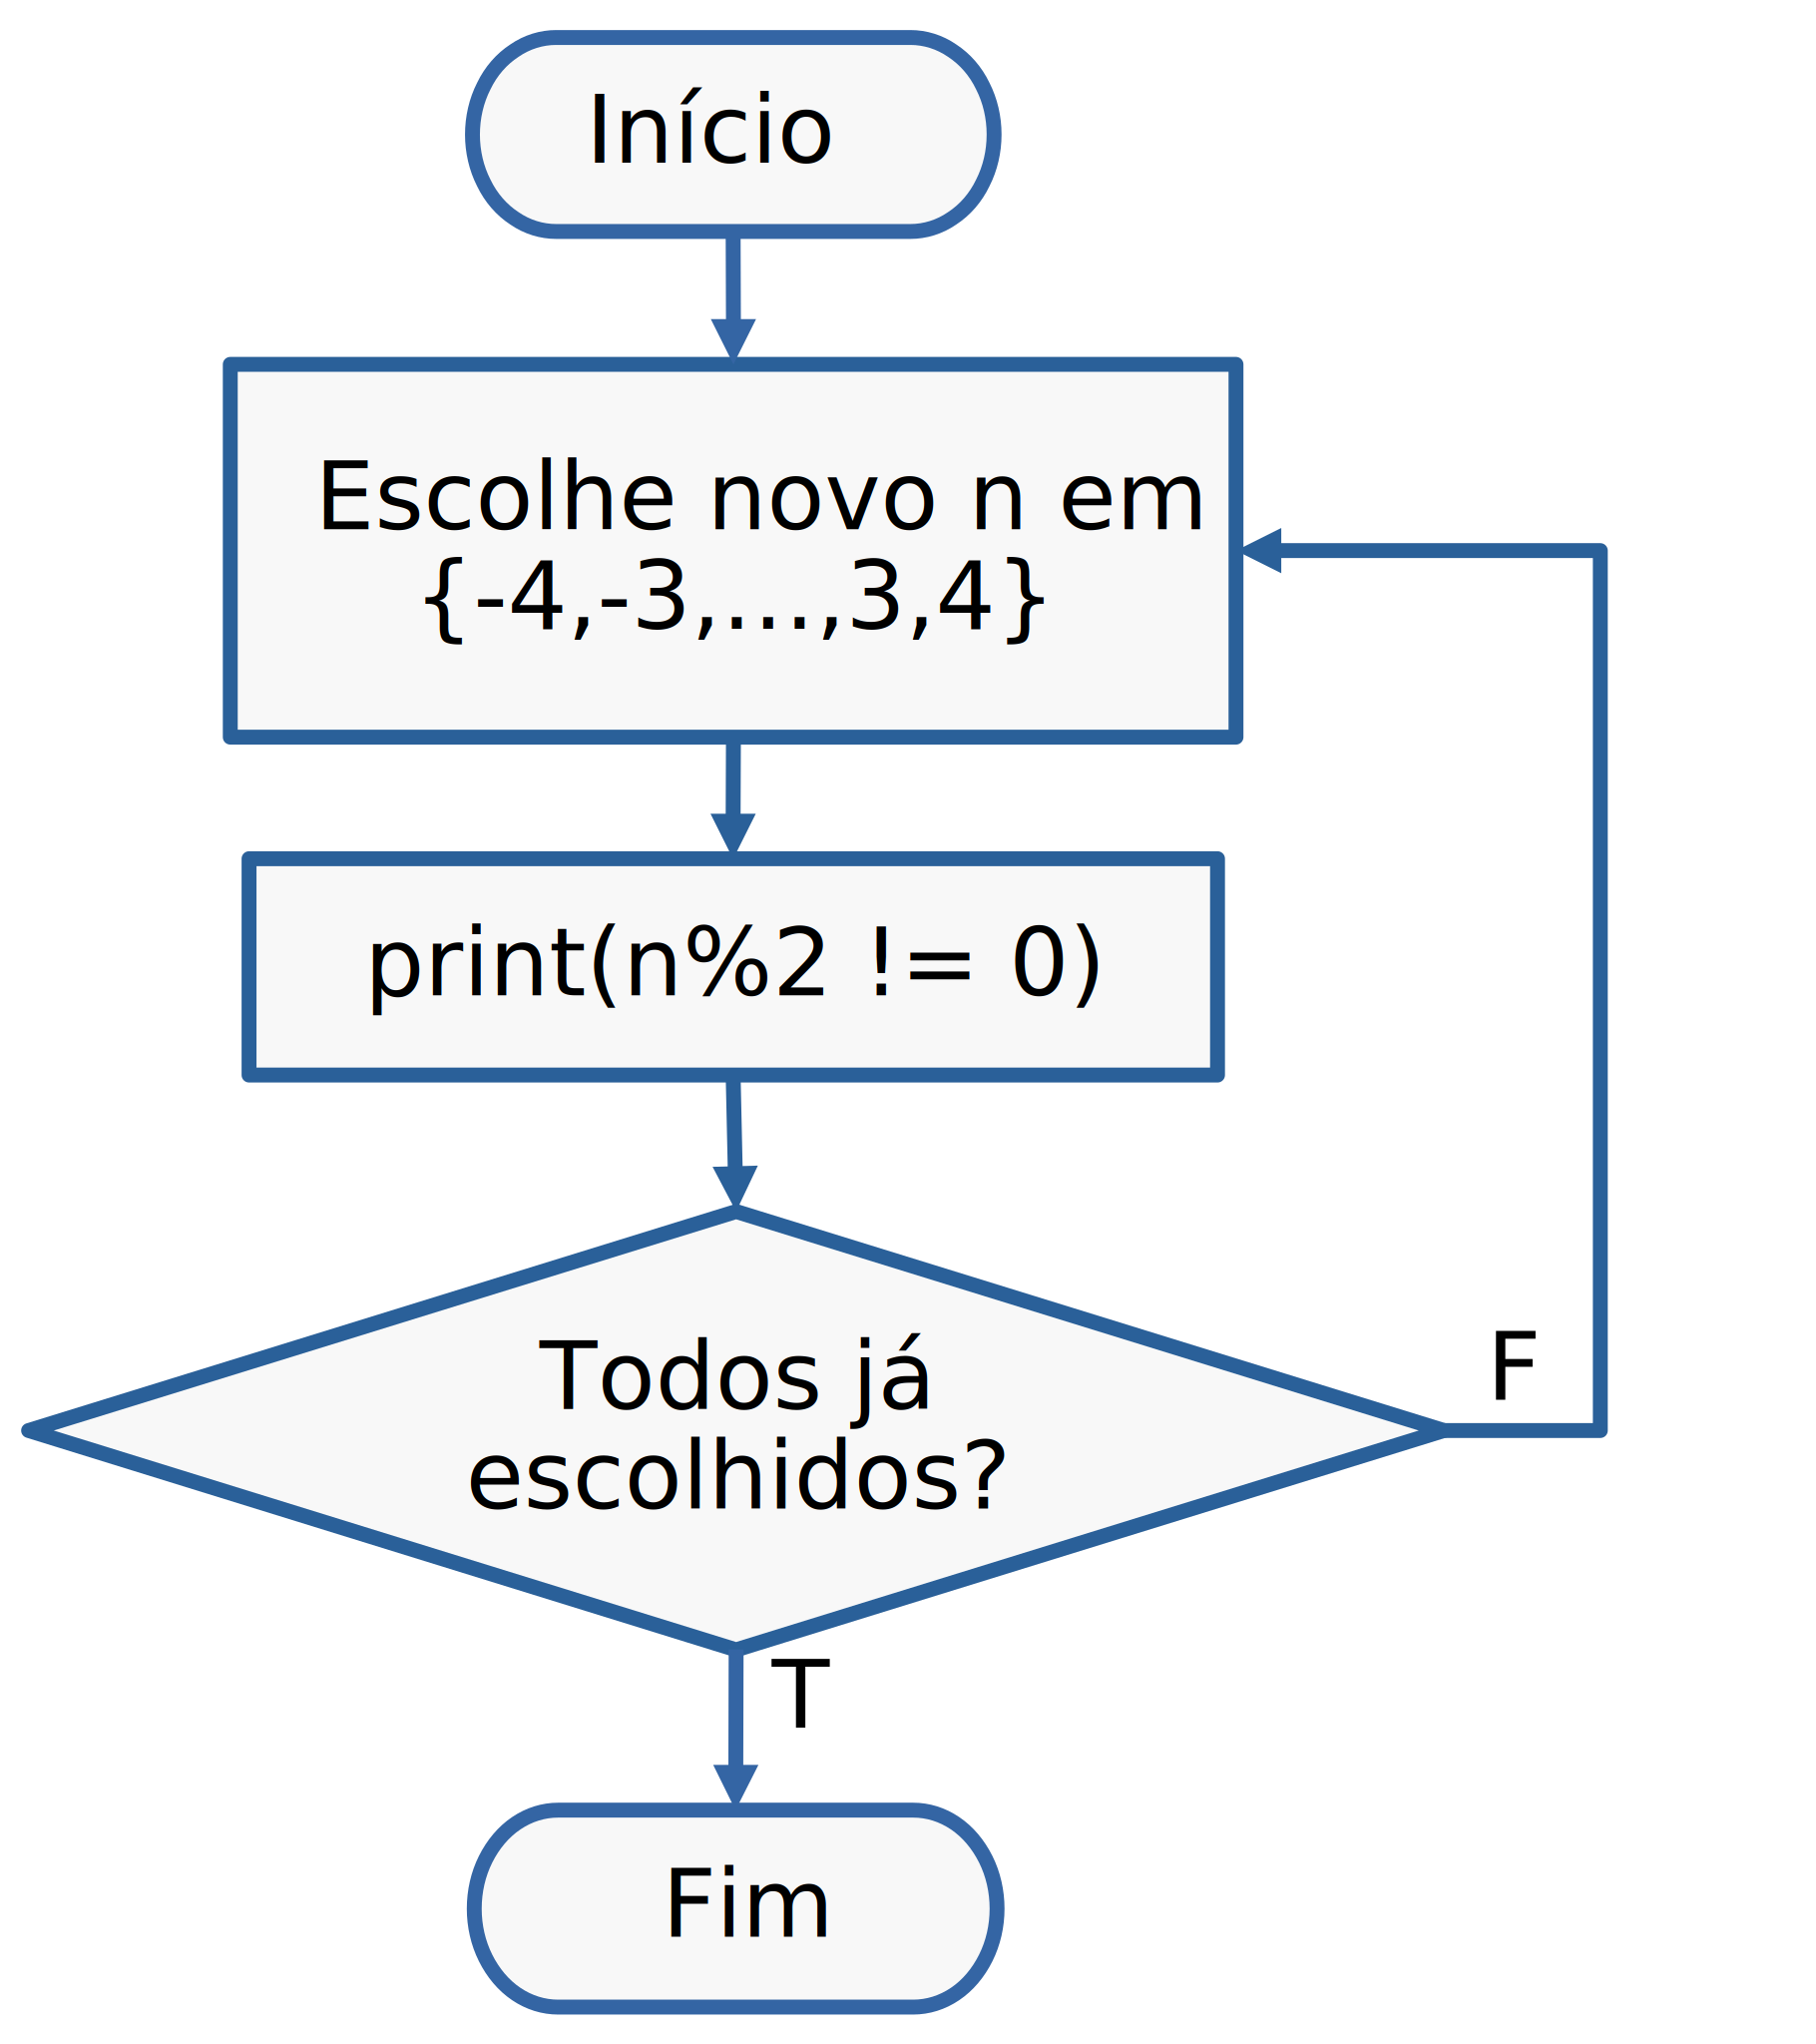
\includegraphics{./cap_lingua/dados/fig_fluxograma/fig}
    \end{center}

  \item {\bf Código {\python}}

\begin{lstlisting}[caption=metHeron.py,label=cap_lingua_sec_algoprog:cod:metHeron]
x = float(input('Entre com o valor de x: '))
if (x >= 0.):
    s = x/2
    for i in range(4):
        s = (s + x/s)/2
    print(f'Raiz aprox. de x = {s}')
else:
    print(f'Não existe!')
\end{lstlisting}
  \end{itemize}
\end{ex}

Algoritmos escritos em uma forma próxima de uma linguagem computacional são, também, chamados de \emph{pseudocódigos}. Na prática, pseudocódigos e fluxogramas são usados para apresentar uma forma mais geral e menos detalhada de um algoritmo. Usualmente, sua forma detalhada é escrita diretamente em uma linguagem computacional escolhida.

\subsection{Exercícios}

\begin{exer}
  Escreva um algoritmo/pseudocódigo e um fluxograma correspondente para o calcular a média aritmética entre dois números $x$ e $y$ dados. Como desafio, tente escrever um código {\python} baseado em seu algoritmo.
\end{exer}

\begin{exer}
  Escreva um algoritmo/pseudocódigo e um fluxograma correspondente para o calcular a área de um quadrado de lado $l$ dado. Como desafio, tente escrever um código {\python} baseado em seu algoritmo.
\end{exer}

\begin{exer}
  Escreva um algoritmo/pseudocódigo e um fluxograma correspondente para o calcular a área de um retângulo de lados $a, b$ dados. Como desafio, tente escrever um código {\python} baseado em seu algoritmo.
\end{exer}

\begin{exer}
  Escreva um algoritmo/pseudocódigo e um fluxograma correspondente para o calcular triângulo retângulo de hipotenusa $h$ e um dos lados $l$ dados. Como desafio, tente escrever um código {\python} baseado em seu algoritmo.
\end{exer}

\begin{exer}
  Escreva um algoritmo/pseudocódigo e um fluxograma correspondente para o calcular o zero de uma função afim
  \begin{equation}
    f(x) = ax + b
  \end{equation}
  dados, os coeficientes $a$ e $b$. Como desafio, tente escrever um código {\python} baseado em seu algoritmo.
\end{exer}

\begin{exer}
  Escreva um algoritmo/pseudocódigo e um fluxograma correspondente para o calcular as raízes reais de um polinômio quadráticos
  \begin{equation}
    p(x) = ax^2 + bx + c
  \end{equation}
  dados, os coeficientes $a$, $b$ e $c$. Como desafio, tente escrever um código {\python} baseado em seu algoritmo.
\end{exer}

\begin{exer}
  A \href{https://pt.wikipedia.org/wiki/S\%C3\%A9rie\_harm\%C3\%B3nica\_(matem\%C3\%A1tica)}{Série Harmônica} é defina por
  \begin{equation}
    \sum_{k=1}^\infty\frac{1}{k} := \frac{1}{1} + \frac{1}{2} + \frac{1}{3} + \cdots
  \end{equation}
  Escreva um algoritmo/pseudocódigo e um fluxograma corresponde para calcular o valor da série harmônica truncada em $k=n$, com $n$ dado. Ou seja, dado $n$, o objetivo é calcular
  \begin{equation}
    \sum_{k=1}^n\frac{1}{k} := \frac{1}{1} + \frac{1}{2} + \cdots + \frac{1}{n}.
  \end{equation}
\end{exer}

\begin{exer}
  O \href{https://pt.wikipedia.org/wiki/E\_(constante\_matem\%C3\%A1tica)}{número de Euler}{\euler} pode ser definido pela série
  \begin{align}
    e &:= \sum_{k=0}^\infty\frac{1}{k!}\\
      &= \frac{1}{0!} + \frac{1}{1!} + \frac{1}{2!} + \frac{1}{3!} + \frac{1}{4!} + \cdots
  \end{align}
  Escreva um algoritmo/pseudocódigo e um fluxograma corresponde para calcular o valor aproximado de $e$ dado pelo truncamento da série em $k=4$, i.e. o objetivo é de calcular
  \begin{align}
    e &\approx \sum_{k=0}^4\frac{1}{k!}\\
      &= \frac{1}{0!} + \frac{1}{1!} + \frac{1}{2!} + \frac{1}{3!} + \frac{1}{4!}\\
      &= \frac{1}{1} + \frac{1}{1} + \frac{1}{1\cdot 2} + \frac{1}{1\cdot 2\cdot 3} + \frac{1}{1\cdot 2\cdot 3\cdot 4}.
  \end{align}
\end{exer}